% utf-8 ru, unix eolns
\documentclass[12pt,a4paper,oneside]{extarticle}
    \righthyphenmin=2 %минимально переносится 2 символа %%%
    \sloppy

% Рукопись оформлена в соответствии с правилами оформления 
% электронной версии авторского оригинала, 
% принятыми в Издательстве МГТУ им. Н.Э. Баумана.

\usepackage{geometry} % А4, примерно 28-31 строк(а) на странице 
    \geometry{paper=a4paper}
    \geometry{includehead=false} % Нет верх. колонтитула
    \geometry{includefoot=true}  % Есть номер страницы
    \geometry{bindingoffset=0mm} % Переплет    : 0  мм
    \geometry{top=20mm}          % Поле верхнее: 20 мм
    \geometry{bottom=25mm}       % Поле нижнее : 25 мм 
    \geometry{left=25mm}         % Поле левое  : 25 мм
    \geometry{right=25mm}        % Поле правое : 25 мм
    \geometry{headsep=10mm}  % От края до верх. колонтитула: 10 мм
    \geometry{footskip=20mm} % От края до нижн. колонтитула: 20 мм 

\usepackage{cmap}
\usepackage[T2A]{fontenc} 
\usepackage[utf8x]{inputenc}
\usepackage[english,russian]{babel}
\usepackage{misccorr}

\usepackage{amsmath}
\usepackage{amsfonts}
\usepackage{amssymb}

%\usepackage{cm-super} %человеческий рендер русских шрифтов

\setlength{\parindent}{1.25cm}  % Абзацный отступ: 1,25 см
\usepackage{indentfirst}        % 1-й абзац имеет отступ

\usepackage{setspace}   

\onehalfspacing % Полуторный интервал между строками

\makeatletter
\renewcommand{\@oddfoot }{\hfil\thepage\hfil} % Номер стр.
\renewcommand{\@evenfoot}{\hfil\thepage\hfil} % Номер стр.
\renewcommand{\@oddhead }{} % Нет верх. колонтитула
\renewcommand{\@evenhead}{} % Нет верх. колонтитула
\makeatother

\usepackage{fancyvrb}


\usepackage[pdftex]{graphicx}  % поддержка картинок для пдф
\graphicspath{ {./pictures/} }
\usepackage{rotating}
%\DeclareGraphicsExtensions{.jpg,.png}




\renewcommand{\labelenumi}{\theenumi.} %меняет вид нумерованного списка

\usepackage{perpage} %нумерация сносок 
\MakePerPage{footnote}

\usepackage[all]{xy} %поддержка графов

\usepackage{listings} %листинги


\usepackage{url}


\usepackage{tikz} %для рисования графиков
\usepackage{pgfplots}

\usepackage{gensymb}

\usepackage{ccaption}%изменяет подпись к рисунку
\makeatletter 
\renewcommand{\fnum@figure}[1]{Рисунок~\thefigure~---~\sffamily}
\makeatother

\begin{document}
\pgfplotsset{compat=1.8}

\thispagestyle{empty}
\newpage
{
\centering


\textbf{
МОСКОВСКИЙ ГОСУДАРСТВЕННЫЙ ТЕХНИЧЕСКИЙ УНИВЕРСИТЕТ ИМЕНИ Н. Э. БАУМАНА \\
Факультет информатики и систем управления \\
Кафедра теоретической информатики и компьютерных технологий}
\bigskip
\bigskip
\bigskip
\bigskip
\bigskip
\bigskip
\bigskip

\vfill


Лабораторная работа №2 \\
по курсу <<Моделирование>>

\bigskip

{\large <<Cравнительный анализ методов решения СЛАУ (метод Гаусса, метод Зейделя)>>}
\bigskip

\vfill



\hfill\parbox{4cm} {
Выполнил:\\
студент ИУ9-91 \hfill \\
Выборнов А. И.\hfill \medskip\\
Руководитель:\\
Домрачева А. Б.\hfill
}


\vspace{\fill}

Москва \number\year
\clearpage
}



\clearpage


\section{Постановка задачи}
    Провести сравнительный анализ методов Гаусса и Зейделя для решения СЛАУ. Реализовать оба метода.

    Под решением СЛАУ подразумевается решение системы уравнений $Ax=b$ показанной на рисунке~\ref{pic:gaussian0}.
    \begin{figure}[h!]
        \centering
        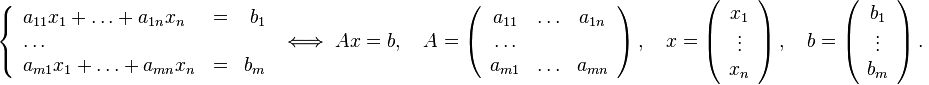
\includegraphics[scale=0.5]{gaussian0.png}
        \caption{Постановка задачи решения СЛАУ}
        \label{pic:gaussian0}
    \end{figure}    
\section{Теоретическая часть}
    \subsection{Метод Гаусса}
        {\it Метод Гаусса}~---~классический метод решения системы линейных алгебраических уравнений. Метод заключается в последовательном исключении переменных и происходит в два этапа:
        \begin{enumerate}
            \item Прямой ход~---~путём элементарных преобразований над строками систему приводят к ступенчатой или треугольной форме, либо устанавливают, что система несовместна.

                На рисунке~---~\ref{pic:gaussian1} показана СЛАУ, приведённая к ступенчатому виду. Количество базисных переменных равно рангу матрицы $A$, то есть будет $r$ базисные переменных. Пусть базисные будут переменные $x_{j_1}, ..., x_{j_r}$, остальные будем называть свободными (небазисными). 
                \begin{figure}[h!]
                    \centering
                    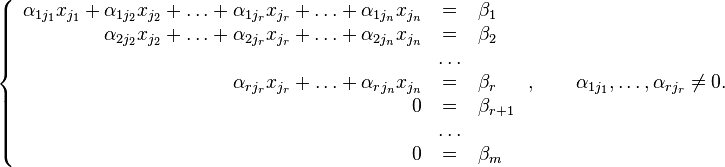
\includegraphics[scale=0.65]{gaussian1.png}
                    \caption{CЛАУ приведённая к ступенчатому виду}
                    \label{pic:gaussian1}
                \end{figure}

                Если $\exists \beta_i \neq 0 \colon i>r$, то рассматриваемая система не совместна, то есть не имеет решений. Если рассматриваемая система совместна, то переходим к следующему этапу.

            \item Обратный ход~---~необходимо выразить все получившиеся базисные переменные через небазисные и построить фундаментальную систему решений, либо, если все переменные являются базисными, то выразить в численном виде единственное решение системы линейных уравнений

                На рисунке~\ref{pic:gaussian2} показана СЛАУ, в которой базисные переменные выражены через свободные.
                \begin{figure}[h!]
                    \centering
                    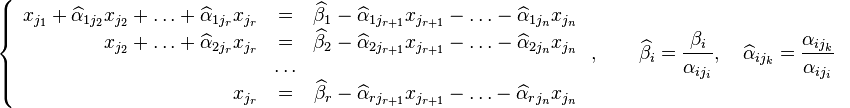
\includegraphics[scale=0.45]{gaussian2.png}
                    \caption{СЛАУ, в которой базисные переменные выражены через свободные}
                    \label{pic:gaussian2}
                \end{figure}

                Если все переменные базисные~---~то получаем единственное решение системы путём последовательного нахождения переменных двигаясь по СЛАУ снизу вверх. Если присутствуют свободные переменные, то мы получаем бесконечное множество решений: перебираем всевозможные значения свободных переменных и находим базисные двигаясь снизу вверх.
        \end{enumerate}

        \subsubsection{Преимущества}
            \begin{itemize}
                \item Для матриц ограниченного размера менее трудоёмкий по сравнению с другими методами.
                \item Позволяет однозначно установить, совместна система или нет, и если совместна, найти её решение.
                \item Позволяет найти ранг матрицы
            \end{itemize}
        \subsubsection{Недостатки}
            \begin{itemize}
                \item Не оптимален - работает за $O(n^3)$: существуют алгоритмы перемножения матриц работающие ассимптотически быстрее.
                \item Вычислительно неустойчив для плохо обусловленных матриц.
            \end{itemize}



    \subsection{Метод Зейделя}
        {\it Метод Зейделя}~---~итерационный метод решения системы линейных уравнений.
        
            Рассмотрим матрицу $A$ размера $n\times n$. Полагаем, что диагональные коэффициенты не нулевые, то есть $\forall i ~a_{ii}\neq 0$. Теперь решаем $i$-ое уравнение относительно $x_i$: 
            $$x_i = \frac{b_i-(a_{i1}x_1 + ... + a_{i(i-1)}x_{i-1} + a_{i(i+1)}x_{i+1} + a_{in}x_n)}{a_{ii}}$$
            Найдя $x_i$ для каждого $i$ получаем систему:
            \begin{equation*}
                \begin{cases}
                    x_1 = \frac{b_1-(a_{12}x_2 + a_{13}x_3 + a_{1n}x_n)}{a_{11}}, \\
                    x_2 = \frac{b_2-(a_{11}x_1 + a_{13}x_3 + a_{1n}x_n)}{a_{22}}, \\
                    ... \\
                    x_n = \frac{b_n-(a_{11}x_1 + a_{12}x_2 + a_{1(n-1)}x_{n-1})}{a_{nn}}. \\
                \end{cases}
            \end{equation*}

            Возьмём некоторый начальный вектор $x^{(0)}$. Подставив его в полученную систему мы получим $x^{(1)}$. Аналогично с помощью $x^{(1)}$ находим $x^{(2)}$. Если будем учитывать полученные ранее решения, то система примет вид:
            \begin{equation*}
                \begin{cases}
                    x_1^{(k+1)} = \frac{b_1-(a_{12}x_2^{(k)} + a_{13}x_3^{(k)} + a_{1n}x_n^{(k)})}{a_{11}}, \\
                    x_2^{(k+1)} = \frac{b_2-(a_{11}x_1^{(k+1)} + a_{13}x_3^{(k)} + a_{1n}x_n^{(k)})}{a_{22}}, \\
                    ... \\
                    x_n^{(k+1)} = \frac{b_n-(a_{11}x_1^{(k+1)} + a_{12}x_2^{(k+1)} + a_{1(n-1)}x_{n-1}^{(k+1)})}{a_{nn}}. \\
                \end{cases}
            \end{equation*}

             Повторяя этот итерационный процесс получаем последовательность приближений: $(x^{(0)}, x^{(1)}, ... , x^{(k)}, ...)$. Если эта последовательность сходится, то $x=\lim_{k \to \infty}x^k$ - является решением системы.

             Разложим матрицу $A$ на сумму матриц $A=L+D+U$, где $D$~---~ диагональная матрица, а матрицы $L$ и $U$ соответственно нижне и верхне диагоальные матрицы. Тогда необходимое условие сходимости метода Зейделя можно записать в виде: \\если $||-(L+D)^{-1}U||<1$, то метод Зейделя сходится.

        \subsubsection{Преимущества}
            \begin{itemize}
                \item Быстро сходится.
                \item Сходимость доказана, всегда можно проверить сходится ли он.
                \item Одна итерация работает за $O(n^2)$, что на больших матрицах даёт преимущество перед методом Гаусса.
            \end{itemize}
        \subsubsection{Недостатки}
            \begin{itemize}
                \item Может медленно сходиться или даже расходиться на некоторых системах.
            \end{itemize}

\section{Реализация}
    В рамках лабораторной работы была написана программа на языке python, которая реализует методы Гаусса и Зейделя

    \subsection{Метод Гаусса}
    Ниже представлена метод на Python, реализующий метод Гаусса. Метод принимает на вход матрицы $A$ и $b$ и возвращает вектор решения $x$.
    \lstset{language=Python}
        \begin{lstlisting}[mathescape] 
    def gaussian(A, b):
        n = len(A)    
        x = [0]*n

        #A = A|b
        A = [A[i]+[b[i]] for i in range(n)]

        for k in range(1, n):
            for j in range(k, n):
                m = A[j][k-1]*1.0 / A[k-1][k-1]
                for i in range(n+1):
                    A[j][i] -= m*A[k-1][i]

        b = [A[i][n] for i in range(n)]

        for i in range(n-1, -1, -1):
            b[i] -= sum(A[i][j]*x[j] for j in range(i+1, n))
            x[i] = b[i]*1.0 / A[i][i]
     
        return x
    \end{lstlisting}

    \subsection{Метод Зейделя}
    Ниже представлена метод на Python, реализующий метод Зейделя. Метод принимает на вход матрицы $A$ и $b$, а также число $eps$, характеризующее точность решения, и возвращает вектор решения $x$.

    \lstset{language=Python}
        \begin{lstlisting}[mathescape] 
    def seidel(A, b, eps):
        n = len(A)

        #Ax=b    
        x = [0] * n
        converge = False
        while not converge:
            p = copy.copy(x)
            for i in range(n):
                s = sum(A[i][j] * x[j] for j in range(i))
                s += sum(A[i][j] * p[j] for j in range(i+1,n))
                x[i] = (b[i] - s)*1.0 / A[i][i]
     
            converge = sqrt(sum((x[i]-p[i])**2 for i in range(n))) < eps
        return x
    \end{lstlisting}

\section{Выводы}
    При реализации на ЭВМ метод Зейделя превосходит метод Гаусса по скорости работы, но требует дополнительной проверки на сходимость. Также, в отличие от метода Гаусса метод Зейделя позволяет находить значения с заданной точностью и уточнять полученные ранее решения.    

\end{document}